\documentclass[a4paper,UTF8]{article}
\usepackage{CJKutf8}
\usepackage[margin=1.25in]{geometry}
\usepackage{color}
\usepackage{graphicx}
\usepackage{amssymb}
\usepackage{amsmath}
\usepackage{amsthm}
\usepackage{multirow}
\usepackage{pdfpages}
\usepackage{tikz}
\usepackage{listings}
\usepackage{xcolor} 
\usepackage{longtable}
\usepackage {ctex}
\usepackage[colorlinks,linkcolor=blue]{hyperref}
\usetikzlibrary{arrows,automata} 
%\setmainfont                    [Ligatures=TeX]{Times New Roman}
\theoremstyle{definition}
\newtheorem*{solution}{Solution}
\newtheorem*{prove}{Proof}
\lstset{
	numbers=left, 
	numberstyle=\tiny,
	basicstyle =\small,
	frame=shadowbox, 
	breaklines=true, 
	showspaces=false,
 	keywordstyle=\color{purple}\bfseries,
	%identifierstyle=\color{brown!80!black},
 	commentstyle=\color{gray}
	stringstyle=\color{brown!60!black},
	rulesepcolor=\color{red!20!green!20!blue!20}
}

\begin{document}
\begin{CJK}{UTF8}{gkai}

\title{\heiti《数据库概论》实验二 高级SQL 实验报告}
\author{
	\songti 姓名: 傅小龙  学号: 191220029  联系方式: 1830970417(QQ)
}
%\date{\color{red} \Large Due: Nov. 30, 2021}
\date{}
\maketitle

\setlength{\baselineskip}{18pt}
\begin{flushleft}
\begin{CJK*}{UTF8}{heiti}
\section*{一、实验环境}
\end{CJK*}
\end{flushleft}
操作系统: Windows 10\\
Mysql Workbench 8.0 CE\\
mysql-8.0.19-winx64\\
Vistual Studio 2019(Community)\\

\begin{flushleft}
\begin{CJK*}{UTF8}{gbsn}
\section*{二、实验过程}
\end{CJK*}
\end{flushleft}

{\heiti \large 任务1-(1):}
\begin{lstlisting}[language=SQL]
drop procedure if exists gen_pruduct_sell_list;
delimiter //
create procedure gen_pruduct_sell_list(in pName Varchar(40))
begin
	select C.customerName, O.orderNo, OD.quantity, OD.price
    from Product P, Customer C, ordermaster O, orderdetail OD
    where P.productNo = OD.productNo and C.customerNo = O.customerNo and O.orderNo = OD.orderNo and P.productName = pName
    order by OD.price desc;
end;
//
call gen_pruduct_sell_list('32M DRAM');
\end{lstlisting}
\par 运行结果详见图1.
\begin{figure}[h]
\centering
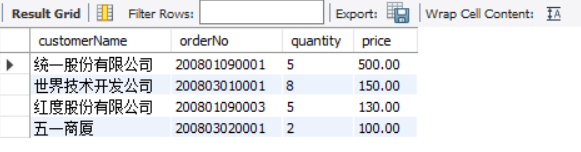
\includegraphics[scale=0.6]{./img/1-1.png}
\caption{1-(1)运行结果}
\label{fig:label}
\end{figure}

{\heiti \large 任务1-(2):}
\begin{lstlisting}[language=SQL]
drop procedure if exists earlierHired_employee;
delimiter //
create procedure earlierHired_employee(in eNumber Char(8))
begin
	select E.employeeNo, E.employeeName, E.gender, E.hireDate, E.department
    from employee E
    where E.hireDate < (
		select E.hireDate
        from employee E
        where E.employeeNo = eNumber
    ) and E.department = (
		select E.department
        from employee E
        where E.employeeNo = eNumber
    );
end
//
call earlierHired_employee('E2008005');
\end{lstlisting}
\par 运行结果详见图2.
\begin{figure}[h]
\centering
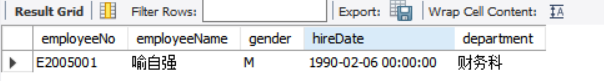
\includegraphics[scale=0.6]{./img/1-2.png}
\caption{1-(2)运行结果}
\label{fig:label}
\end{figure}

{\heiti \large 任务2-(1):}
\begin{lstlisting}[language=SQL]
drop function if exists avg_order_price;
delimiter //
create function avg_order_price(pName Varchar(40))
returns float
DETERMINISTIC
begin
	declare avg_price float;
	select avg(OD.price) into avg_price
    from orderdetail OD, Product P
    where OD.productNo = P.productNo and P.productName = pName
    group by P.productName;
    return avg_price;
end;
//
select P.productName, avg_order_price(P.productName)
from Product P;
\end{lstlisting}
\par 运行结果详见图3.
\begin{figure}[h]
\centering
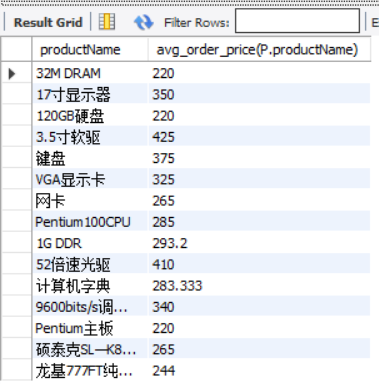
\includegraphics[scale=0.6]{./img/2-1.png}
\caption{2-(1)运行结果}
\label{fig:label}
\end{figure}

{\heiti \large 任务2-(2):}
\begin{lstlisting}[language=SQL]
drop function if exists sum_product_sell;
delimiter //
create function sum_product_sell(pNo char(9))
returns integer
DETERMINISTIC
begin
	declare sum_sell integer;
	select sum(OD.quantity) into sum_sell
    from orderdetail OD
    where OD.productNo = pNo
    group by OD.productNo;
    return sum_sell;
end;
//
select P.productNo, P.productName, sum_product_sell(P.productNo)
from Product P
where sum_product_sell(P.productNo) > 4;
\end{lstlisting}
\par 运行结果详见图4.
\begin{figure}[h]
\centering
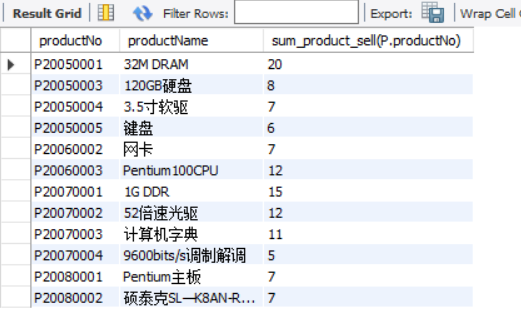
\includegraphics[scale=0.6]{./img/2-2.png}
\caption{2-(2)运行结果}
\label{fig:label}
\end{figure}

{\heiti \large 任务3-(1):}
\begin{lstlisting}[language=SQL]
drop trigger if exists pPrice_insert;
delimiter //
create trigger pPrice_insert before insert on product
	for each row
begin
	if new.productPrice > 1000 then
		set new.productPrice = 1000;
	end if;
end;
\end{lstlisting}
\par 采用如下sql语句进行测试, 运行结果详见图5.可以看到编号为'P20090002'的产品价格被修改为了1000.
\begin{lstlisting}[language=SQL]
insert into product
(productNo, productName, productClass, productPrice)
VALUES
('P20090001', 'test1', 'test', 100),
('P20090002', 'test2', 'test', 12000);
select * from product where productNo like 'P2009%';
delete from product where productNo like 'P2009%';
\end{lstlisting}
\begin{figure}[h]
\centering
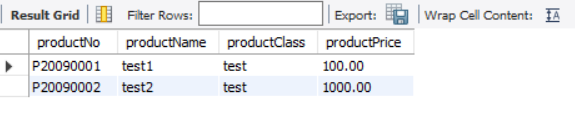
\includegraphics[scale=1]{./img/3-1.png}
\caption{3-(1)运行结果}
\label{fig:label}
\end{figure}

{\heiti \large 任务3-(2):}
\begin{lstlisting}[language=SQL]
drop trigger if exists raise_salary;
delimiter //
create trigger raise_salary before insert on ordermaster
	for each row
begin
	declare old_salary float;
    set old_salary = (
		select salary
        from employee
        where employeeNo = new.employeeNo
    );
	if (
		select hireDate
        from employee
        where employeeNo = new.employeeNo
    ) < date('1992-01-01') then
		update employee set salary = old_salary * 1.08 where employeeNo = new.employeeNo;
	else 
		update employee set salary = old_salary * 1.05 where employeeNo = new.employeeNo;
	end if;
end
\end{lstlisting}
\par 采用如下sql语句进行测试, 运行结果详见图6.可以看到1992年前入职的的'E2021002'员工在完成一个订单后工资增长了8\%, 1992年后入职的'E2021001'员工在完成一个订单后工资增长了5\%, 而没有完成订单的'E2021003'员工工资没有增长.
\begin{lstlisting}[language=SQL]
insert into employee
(employeeNo, employeeName, gender, birthday, address, telephone, hireDate, department, headShip, salary)
VALUES
('E2021001', 'test1', 'M', '1968-01-06', 'test', NULL, '1992-02-28', 'test', 'test', 1000),
('E2021002', 'test2', 'M', '1968-01-06', 'test', NULL, '1991-02-28', 'test', 'test', 1000),
('E2021003', 'test2', 'M', '1968-01-06', 'test', NULL, '1991-02-28', 'test', 'test', 1000);
insert into ordermaster
(orderNo, customerNo, employeeNo, orderDate, orderSum, invoiceNo)
VALUES
('P20210001', 'C20050001', 'E2021001', '2008-01-09', 0, 'I202100001'),
('P20210002', 'C20050001', 'E2021002', '2008-01-09', 0, 'I202100001');

select employeeNo, hireDate, salary
from employee
where employeeNo like 'E2021%';
delete from ordermaster where orderNo like '2021%';
SET FOREIGN_KEY_CHECKS = 0;
delete from employee where employeeNo like 'E2021%';
SET FOREIGN_KEY_CHECKS = 1;
\end{lstlisting}
\begin{figure}[h]
\centering
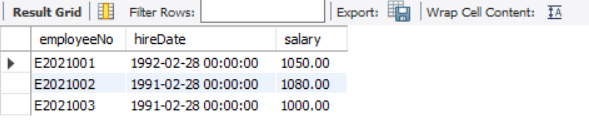
\includegraphics[scale=0.6]{./img/3-2.png}
\caption{3-(2)运行结果}
\label{fig:label}
\end{figure}


以下内容均采用C++与mySql建立连接:
\begin{lstlisting}[language=C++]
const char user[] = "admin";
    const char pswd[] = "123";
    const char host[] = "localhost";
    const char db[] = "orderdb";
    unsigned int port = 3309;

    MYSQL myConnect;
    MYSQL_RES* result = NULL;
    MYSQL_ROW sql_row;
    int res = 0;
    mysql_init(&myConnect);
    if (mysql_real_connect(&myConnect, host, user, pswd, db, port, NULL, 0)){
		...
	}
\end{lstlisting}
{\heiti \large 任务4-(1):(C++)}
\begin{lstlisting}[language=C++]
char order_4_1[] = "select employeeNo, employeeName, salary from employee order by salary desc limit 20";
        res = mysql_query(&myConnect, order_4_1);
        if (!res)
        {
            result = mysql_store_result(&myConnect);
            if (result)
            {
                int num_fields = mysql_num_fields(result);
                MYSQL_FIELD* field;
                char space[] = "                    ";
                while (field = mysql_fetch_field(result)) {
                    char s[128];
                    sprintf(s, "%s%s", field->name, space);
                    printf("%-20.20s", s);
                }
                cout << endl;
                while (sql_row = mysql_fetch_row(result))
                {
                    for (int i = 0; i < num_fields; i++) {
                        char s[128];
                        sprintf(s, "%s%s", sql_row[i], space);
                        printf("%-20.20s", s);
                    }
                    cout << endl;
                }
            }
        }
        else
        {
            cout << "query sql failed!" << endl;
        }
\end{lstlisting}
\par 运行结束后的控制台输出如图7所示.
\begin{figure}[h]
\centering
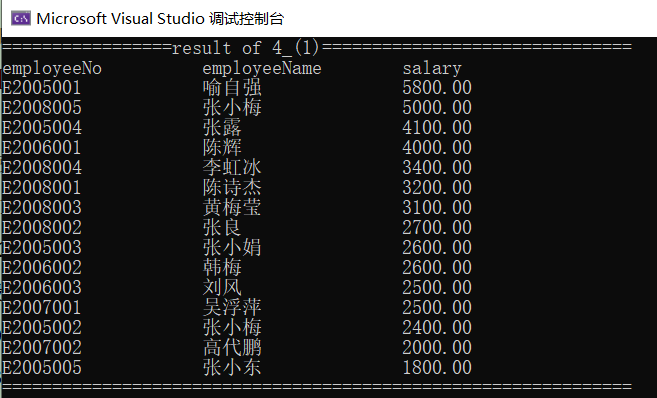
\includegraphics[scale=0.8]{./img/4-1.png}
\caption{4-(1)运行结果}
\label{fig:label}
\end{figure}

{\heiti \large 任务4-(2):(C++)}
\begin{lstlisting}[language=C++]
char order_4_2[] = "insert into customer(customerNo, customerName, address, telephone, zip) values ('C20080002', '********', '***', '010-5422685', '220501')";
        printf(fence_begin, 4, 2);
        res = mysql_query(&myConnect, order_4_2);
        if (!res)
        {
            cout << "query sql succeeded!" << endl;;
        }
        else
        {
            cout << "query sql failed!" << endl;
        }
\end{lstlisting}
\par 上面代码块中中文内容未能正常显示. 变量order\_4\_2的值为"insert into customer(customerNo, customerName, address, telephone, zip) values ('C20080002', '泰康股份有限公司', '天津市', '010-5422685', '220501')".
\par 运行结束后的控制台输出以及在mySql中查询客户ID为'C20080002'的结果如图8所示.
\begin{figure}[h]
\centering
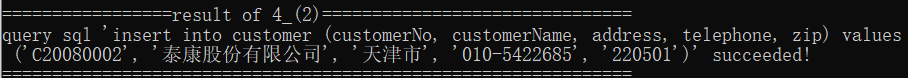
\includegraphics[scale=0.7]{./img/4-2-1.png}
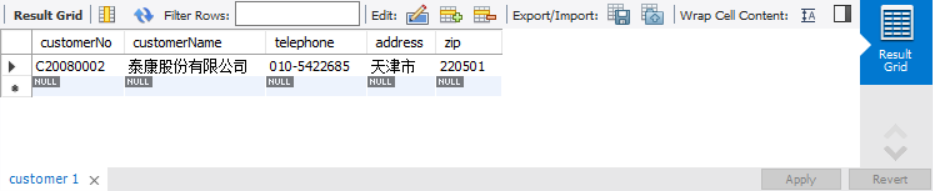
\includegraphics[scale=0.7]{./img/4-2-2.png}
\caption{4-(2)运行结果}
\label{fig:label}
\end{figure}

{\heiti \large 任务4-(3):(C++)}
\begin{lstlisting}[language=C++]
char order_4_3[5][128] = { "SET FOREIGN_KEY_CHECKS = 0",
                            "SET SQL_SAFE_UPDATES = 0",
                            "delete from employee where salary > 5000",
                            "SET SQL_SAFE_UPDATES = 1;",
                            "SET FOREIGN_KEY_CHECKS = 1" };
        for (int i = 0; i < 5; i++) {
            res = mysql_query(&myConnect, order_4_3[i]);
            if (!res)
            {
                cout << "query sql '" << order_4_3[i] << " 'succeeded!" << endl;;
            }
            else
            {
                cout << "query sql'" << order_4_3[i] << " ' failed!" << endl;
                break;
            }
        }
\end{lstlisting}
\par 运行结束后的控制台输出以及在删除语句执行前后mySql中查询薪水高于5000的员工信息如图9所示.
\begin{figure}[h]
\centering
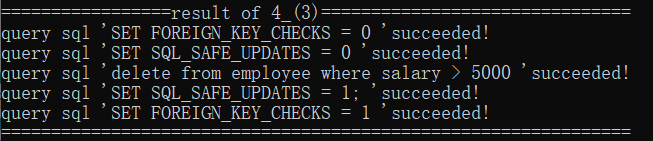
\includegraphics[scale=0.7]{./img/4-3-1.png}
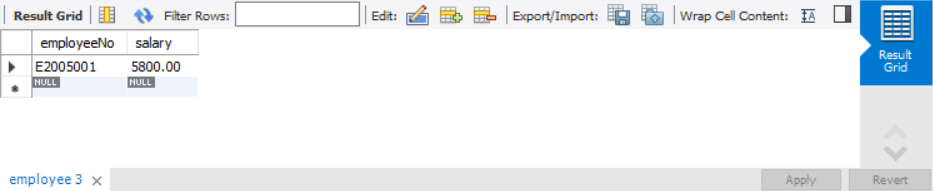
\includegraphics[scale=0.6]{./img/4-3-2.png}
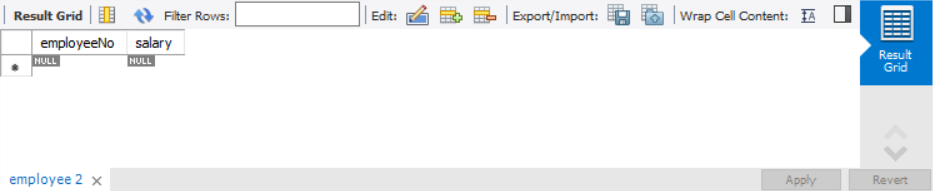
\includegraphics[scale=0.6]{./img/4-3-3.png}
\caption{4-(3)运行结果}
\label{fig:label}
\end{figure}

{\heiti \large 任务4-(4):(C++)}
\begin{lstlisting}[language=SQL]
char order_4_3[3][128] = { "SET SQL_SAFE_UPDATES = 0",
                                "update product set productPrice = productPrice * 0.5 where productPrice > 1000",
                                "SET SQL_SAFE_UPDATES = 1" };
        for (int i = 0; i < 3; i++) {
            res = mysql_query(&myConnect, order_4_3[i]);
            if (!res)
            {
                cout << "query sql '" << order_4_3[i] << " 'succeeded!" << endl;;
            }
            else
            {
                cout << "query sql'" << order_4_3[i] << " ' failed!" << endl;
                break;
            }
        }
\end{lstlisting}
\par 运行结束后的控制台输出以及在更新语句执行前后mySql中商品价格高于1000的商品信息如图10所示.
\begin{figure}[h]
\centering
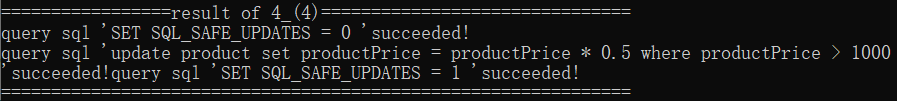
\includegraphics[scale=0.7]{./img/4-4-1.png}
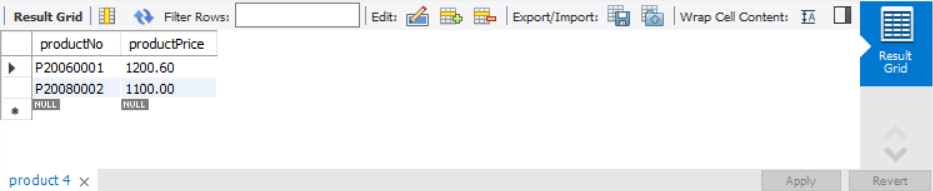
\includegraphics[scale=0.6]{./img/4-4-2.png}
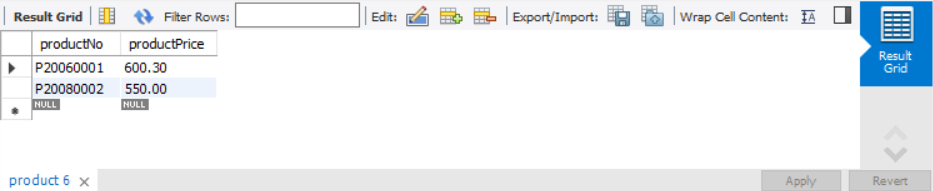
\includegraphics[scale=0.6]{./img/4-4-3.png}
\caption{4-(4)运行结果}
\label{fig:label}
\end{figure}

{\heiti \large 任务5-(1):(C++)}
\begin{lstlisting}[language=C++]
char order_5_1[6][128] =  { "SET SQL_SAFE_UPDATES = 0",
"set @sql = \"update employee set salary = salary + 200 where department = '",
"PREPARE stmt FROM @sql",
"EXECUTE stmt",
"deallocate prepare stmt",
"SET SQL_SAFE_UPDATES = 1" };
        char department[128];
        cout << "Please input department Name:";
        cin >> department;
        strcat(department, "'");
        strcat(order_5_1[1], department);
        for (int i = 0; i < 6; i++) {
            res = mysql_query(&myConnect, order_5_1[i]);
            if (!res)
            {
                cout << "query sql '" << order_5_1[i] << " 'succeeded!" << endl;;
            }
            else
            {
                cout << "query sql'" << order_5_1[i] << " ' failed!" << endl;
                break;
            }
        }
\end{lstlisting}
\par 运行结束后的控制台输出以及在更新语句执行前后mySql中业务科员工工资信息如图11所示.
\begin{figure}[h]
\centering
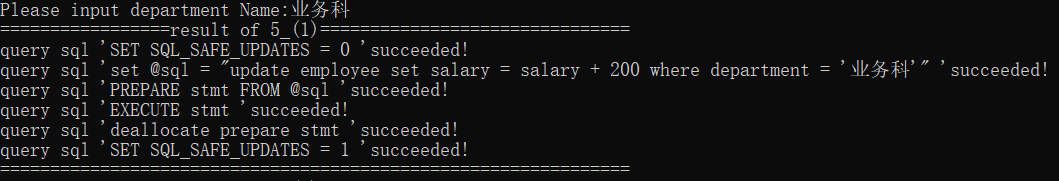
\includegraphics[scale=0.7]{./img/5-1-1.png}
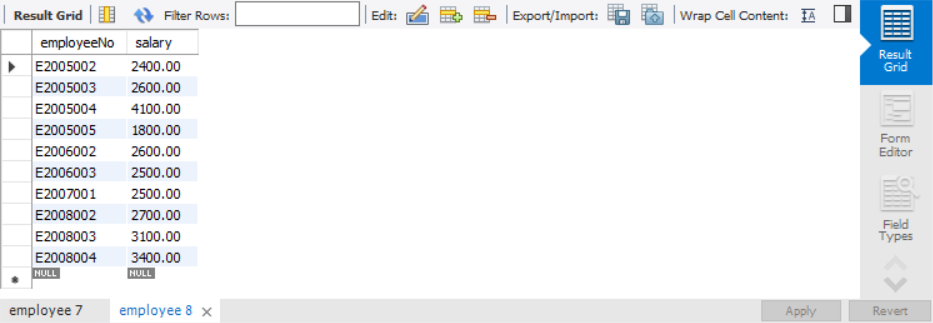
\includegraphics[scale=0.6]{./img/5-1-2.png}
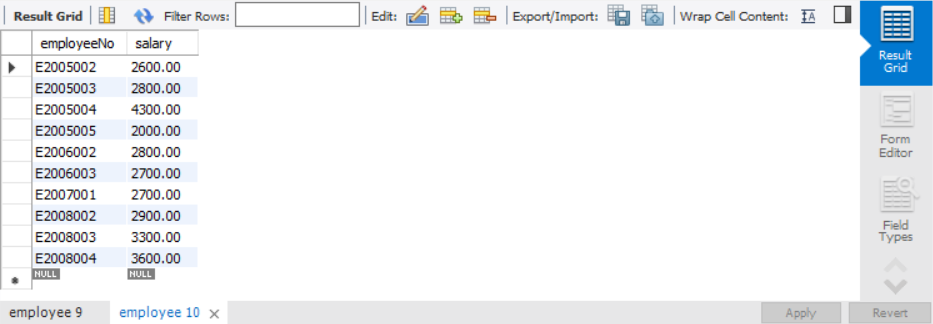
\includegraphics[scale=0.6]{./img/5-1-3.png}
\caption{5-(1)运行结果}
\label{fig:label}
\end{figure}

{\heiti \large 任务5-(2):(C++)}
\begin{lstlisting}[language=C++]
char order_5_2[1][128] = { "select customerName, address, telephone from customer" };
        for (int i = 0; i < 1; i++) {
            res = mysql_query(&myConnect, order_5_2[i]);
            if (!res)
            {
                result = mysql_store_result(&myConnect);
                    if (result)
                    {
                        int num_fields = mysql_num_fields(result);
                        MYSQL_FIELD* field;
                        char space[] = "                    ";
                        while (field = mysql_fetch_field(result)) {
                            char s[128];
                            sprintf(s, "%s%s", field->name, space);
                            printf("%-30.30s", s);
                        }
                        cout << endl;
                        while (sql_row = mysql_fetch_row(result))
                        {
                            for (int i = 0; i < num_fields; i++) {
                                char s[128];
                                sprintf(s, "%s%s", sql_row[i], space);
                                printf("%-30.30s", s);
                            }
                            cout << endl;
                        }
                    }

            }
            else
            {
                cout << "query sql'" << order_5_2[i] << " ' failed!" << endl;
                cout << mysql_error(&myConnect);
                break;
            }
        }
\end{lstlisting}
\par 运行结束后的控制台输出如图12所示.
\begin{figure}[h]
\centering
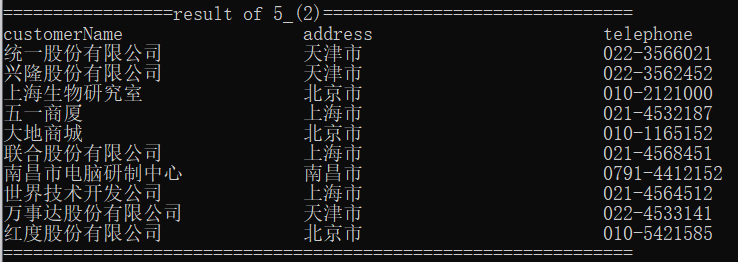
\includegraphics[scale=0.7]{./img/5-2-1.png}
\caption{5-(2)运行结果}
\label{fig:label}
\end{figure}

\begin{flushleft}
\begin{CJK*}{UTF8}{heiti}
\section*{三、实验中遇到的困难及解决办法}
\end{CJK*}
\end{flushleft}
\par 配置C++ MySql时寻找教程$^{1}$花费了一定的时间.\\
\begin{flushleft}
\begin{CJK*}{UTF8}{heiti}
\section*{四、参考文献及致谢}
\end{CJK*}
\end{flushleft}
\begin{enumerate}
\item[1.] \url{https://www.cnblogs.com/justinzhang/archive/2011/09/23/2185963.html}
\end{enumerate}
\end{CJK}
\end{document}